\documentclass[aspectratio=169]{beamer}

% shift figures over so that they fit on the page
\usepackage{changepage}

% put line breaks in table cells
\usepackage{makecell}

% for making columns
\usepackage{multicol}

% include pretty pictures
\usepackage{graphicx}

% for giant question mark
\usepackage{anyfontsize}


\usetheme{PaloAlto}
\usecolortheme{whale}

\title[]{Revamp of High Energy Physics Laboratory's Computer Systems}
\author[]{Josef Bostik \\Eric Pereira \\Ryan Wojtyla}
\date{March 18, 2019}

\begin{document}

%----------BEGIN TITLE----------

\begin{frame}
  \titlepage
\end{frame}

%-----------END TITLE-----------

%----------BEGIN GOALS----------

\section{Milestone 5 Goals}

\begin{frame}
  
  \frametitle{Milestone 5 Progress}

\begin{adjustwidth}{-0.4cm}{}
  \begin{center}
      \begin{tabular}{|c|c|c|c|}
        \hline
        Task & Progress & Notes\\
        \hline
        Continue to Care for Existing MTS & 40\% & \\
        Get Info for MTS Instructions & 50\% & improve upon provided
                                                        instructions \\
        Work on MTS Dev. & 50\% & coax AMORE into building \\
        Integrate Nodes into Cluster & 100\% & NAS-0 and SE still must be
                                               included \\
        Assist Researchers & 100\% & \begin{tabular}{@{}c@{}} helping out with
                                       general\\ problems as they arise \end{tabular} \\
        \hline
    \end{tabular}
  \end{center}
\end{adjustwidth}
  
\end{frame}

%-----------END GOALS-----------

%----------BEGIN GEM COMPUTERS----------

\section{GEM Computers}

\begin{frame}

  \frametitle{GEM Computers}

  \begin{itemize}
    \item Assist the researchers with their computer issues.
      \begin{itemize}
        \item Discovered that many of the lab's computers have an unfortunate
          RAID configuration.
      \end{itemize}
      \item Optimize the researchers' workflows.
        \begin{itemize}
          \item Wrote some brief scripts to enhance data processing.
        \end{itemize}
  \end{itemize}

\end{frame}

%-----------END GEM COMPUTERS-----------

%----------BEGIN CLUSTER----------

\section{Compute Cluster}

\begin{frame}

  \frametitle{Compute Cluster}

  \begin{multicols}{2}

  \begin{itemize}
    \item The nodes and SE have been integrated into the cluster!
      \begin{itemize}
        \item except for one uncooperative node...
      \end{itemize}
    \item NAS-0 still needs to be integrated.
      \begin{itemize}
        \item The OS drive group is not showing up in the Anaconda installer.
      \end{itemize}
  \end{itemize}

  \columnbreak
  
  \begin{figure}[H]
    \begin{center}
      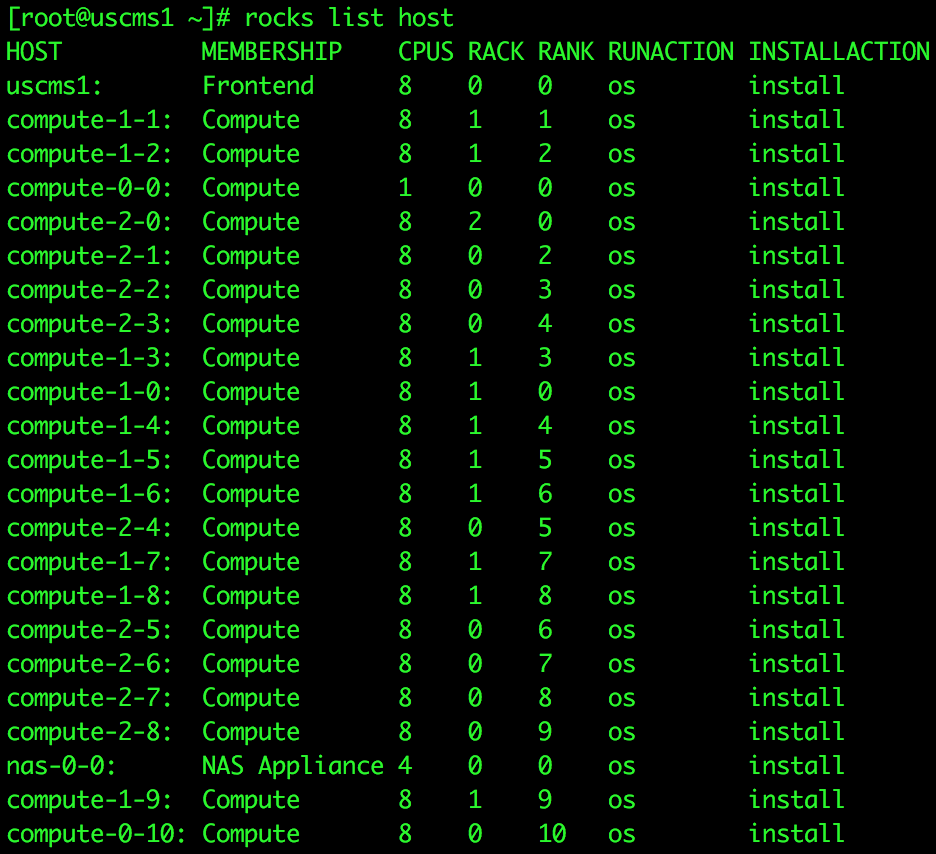
\includegraphics[width=1.0\textwidth]{rocksHostList.png}
    \end{center}
  \end{figure}

  \end{multicols}

\end{frame}

%-----------END CLUSTER-----------

\section{Muon Tomography Station}

%----------BEGIN EXISTING MTS----------

\subsection{Existing MTS}

\begin{frame}

  \frametitle{Existing MTS}

  \begin{itemize}
    \item The FEC with the faulty firmware is still broken.
      \begin{itemize}
        \item We obtained the firmware version that was supposed to work with
          the FEC.
        \item While the firmware installation was successful, the FEC still
          failed to function.
      \end{itemize}
    \item Another, separate FEC has decided to boycott ethernet.
    \item The MTS researchers have been instructed to try to get the remaining,
      functional parts of the detector operational rather than continue trying to
      repair the entire thing.
  \end{itemize}

  % picture of pretty cables

\end{frame}

%-----------END EXISTING MTS-----------

%----------BEGIN DEVELOPMENT MTS----------

\subsection{Development MTS}

\begin{frame}

  \frametitle{Development MTS}

  \begin{itemize}
    \item Attempted to build AMORE from source
    \item Makefile 'Makefile.arch' was not found during build configuration, but
      we did find the file in another directory, and made AMORE reliant on that
      Makefile instead.
    \item Build got further, but a few header files weren't found. The
      configuration seems to not know the proper location to find some files.
    \item Continued attempting to get the previous build of AMORE working, by
    	  manually changing dependencies to our new version of root.
  \end{itemize}

\end{frame}

%-----------END DEVELOPMENT MTS-----------

%----------BEGIN DOCUMENTATION----------

\section{Documentation}

\begin{frame}

  \frametitle{Documentation}

  \begin{itemize}
  \item Documentation is key to the long-term success of the project.
  \item We have been taking extensive notes and recording everything we have
    been doing.
  \item These logs will be compiled into proper manuals.
    \begin{itemize}
    \item step-by-step instructions
    \item troubleshooting
    \end{itemize}
  \end{itemize}
  
  \begin{multicols}{2}
    
    \begin{center}
      
\includegraphics[width=0.5\textwidth]{clusterDoc.png}
    \end{center}

    \columnbreak
    
    \begin{center}
      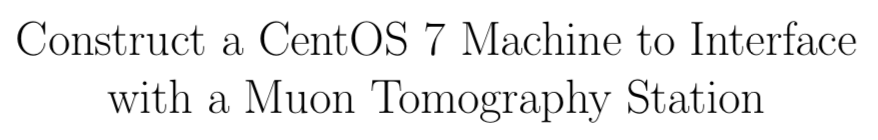
\includegraphics[width=0.5\textwidth]{mtsDoc.png}
    \end{center}

  \end{multicols}

\end{frame}

%-----------END DOCUMENTATION-----------

%----------BEGIN MILESTONE 5 GOALS----------

\section{Milestone 6 Goals}

\begin{frame}

  \frametitle{Milestone 6 Goals}

  \begin{center}
    \begin{tabular}{|c|c|c|c|}
      \hline
      Task & Josef & Eric & Ryan \\
      \hline
      Polish Cluster Documentation & 10\% & 10\% & 80\% \\
      Polish MTS Documentation & 40\% & 20\% & 40\% \\
      Create MTS Automation Script & 60\% & 10\% & 20\% \\
      Integrate Remainder of Cluster Components & 10\% & 10\% & 80\% \\
      Run Jobs on Cluster & 10\% & 10\% & 80\% \\
      Create GEM computer Backups & 10\% & 80\% & 10\% \\
      Assist Researchers & 10\% & 80\% & 10\% \\
      \hline
    \end{tabular}
  \end{center}

\end{frame}

%-----------END MILESTONE 6 GOALS-----------

%----------BEGIN QUESTIONS----------

\section{Questions}

\begin{frame}

  \frametitle{Questions}

  \begin{center}
    {\fontsize{200}{200}\selectfont ?}
  \end{center}
  
\end{frame}

%-----------END QUESTIONS-----------


\end{document}
